\chapter{Integrals}

\section{Change of Variables in Double Integrals}

The new variable $r$ and $\theta$ are related to the old variables $x$ and $y$ by the equations

\begin{align}
    x = r\cos \theta && y = r\sin \theta
\end{align}

We consider a change of variables that is given by a transformation $T$ from the $uv$-plane to the $xy$-plane

\begin{equation}
    T(u, v) = (x, y)
\end{equation}

where $x$ and $y$ are related to $u$ and $v$ by the equations

\begin{align}
    x = g(u, v) && y = h(u, v)
\end{align}

we usually assume that $T$ is a $C^1$ transformation, which means that $g$ and $h$ have continuous first-order partial derivatives.

A transformation $T$ is really just a function whose domain and range are both subsets of $\mathbb{R}^2$.

If $T(u_1, v_1)=(x_1, y_1)$, then the point $(x_1, y_1)$ is called the \textbf{image} of the point $(u_1, v_1)$.

If no two points have the same image, $T$ is called \textbf{one-to-one}.

\begin{figure}
    \centering
    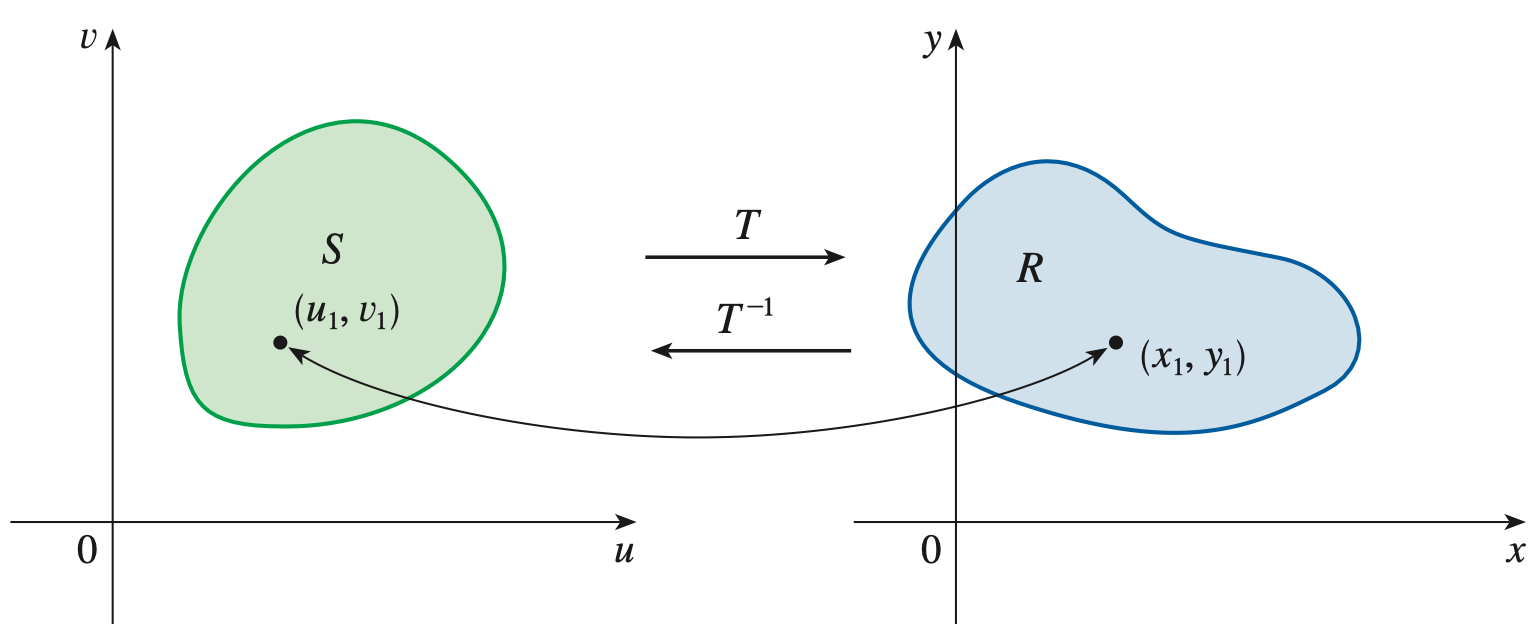
\includegraphics[scale=0.3]{appendices/figures/fig008.png}
    \caption{One-to-one Transformation}
\end{figure}

$T$ transforms $S$ into a region $R$ in the $xy$-plane called the \textbf{image of S}, consisting of the images of all points in $S$.

If $T$ is a one-to-one transformation, then it has an \textbf{inverse transformation} $T^{-1}$ from the $xy$-plane to the $uv$-plane.

\begin{figure}
    \centering
    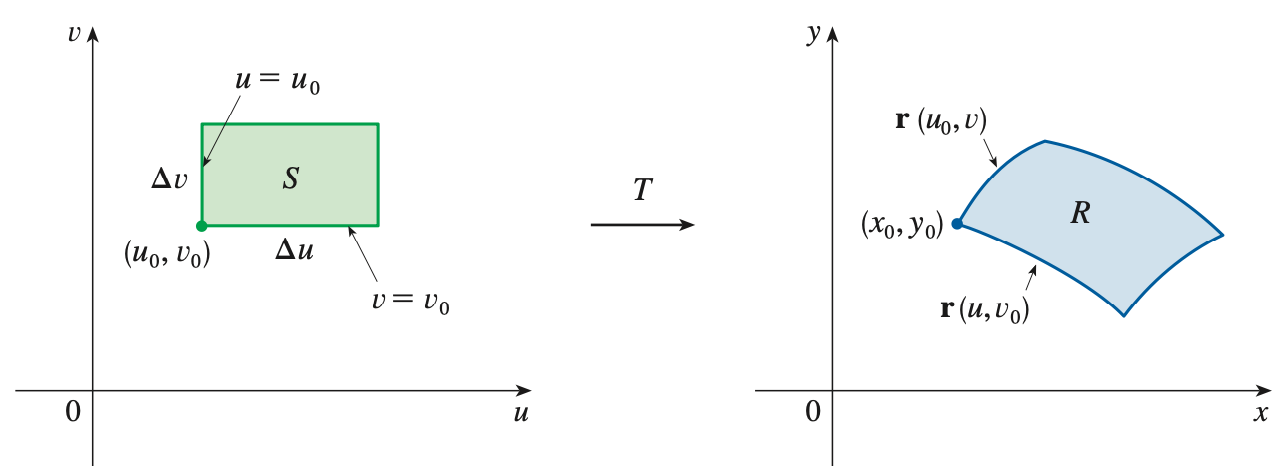
\includegraphics[scale=0.3]{appendices/figures/fig009.png}
    \caption{A change of variables affects a double integral}
\end{figure}

We start with a small rectangle $S$ in the $uv$-plane whose lower left corner is the point $(u_0, v_0)$ and whose dimensions are $\Delta u$ and $\Delta v$.

The image of $S$ is a region $R$ in the $xy$-plane, one of whose boundary points $(x_0, y_0)$ = $T(u_0, v_0)$. The vector $r(u, v)$ is defined as

\begin{equation}
    r(u, v) = g(u, v) \mathbf(i) + h(u, v) \mathbf(j)
\end{equation}

The vector $r(u, v)$ is the position vector of the image of the point $(u, v)$ .

The equation of the lower side of $S$ is $v = v_0$, whose image curve is given by the vector function $r(u, v_0)$. The tangent vector at $(x_0, y_0)$ to this image curve is

\begin{equation}
    r_u = g_u(u_0, v_0)\mathbf{i} + h_u(u_0, v_0)\mathbf{j} = \frac{\partial x}{\partial u}\mathbf{i} + \frac{\partial y}{\partial u}\mathbf{j}
\end{equation}

\begin{figure}
    \centering
    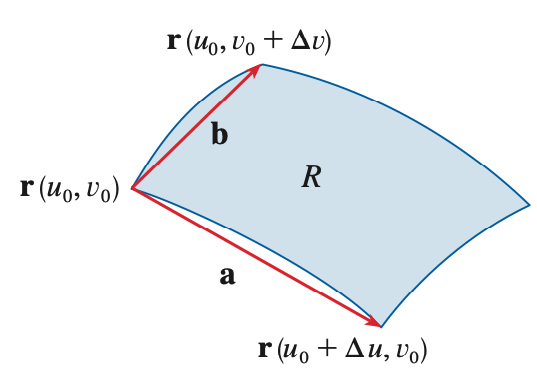
\includegraphics[scale=0.3]{appendices/figures/fig010.png}
    \caption{A change of variables affects a double integral}
\end{figure}

Similarity, the tangent vector at $(x_0, y_0)$ to the image curve of the left side of $S$ is

\begin{equation}
    r_v = g_v(u_0, v_0)\mathbf{i} + h_v(u_0, v_0)\mathbf{j} = \frac{\partial x}{\partial v}\mathbf{i} + \frac{\partial y}{\partial v}\mathbf{j}
\end{equation}

We can approximate the image region $R=T(S)$ by a parallelogram determined by the secant vectors

\begin{align}
    a = r(u_0 + \Delta u, v_0) - r(u_0, v_0) && b = r(u_0, v_0 + \Delta v) - r(u_0, v_0)
\end{align}

but 

\begin{equation}
    r_u = \lim_{\Delta u \rightarrow 0} \frac{r(u_0 + \Delta u, v_0) - r(u_0, v_0)}{\Delta u}
\end{equation}

and so

\begin{equation}
    r(u_0 + \Delta u, v_0) - r(u_0, v_0) \approx \Delta u r_u
\end{equation}

similarity

\begin{equation}
    r(u_0, v_0 + \Delta v) - r(u_0, v_0) \approx \Delta v r_v
\end{equation}

This means that we can approximate $R$ by a parallelogram determined by the vectors $\Delta u r_u$ and $\Delta v r_v$

\begin{figure}
    \centering
    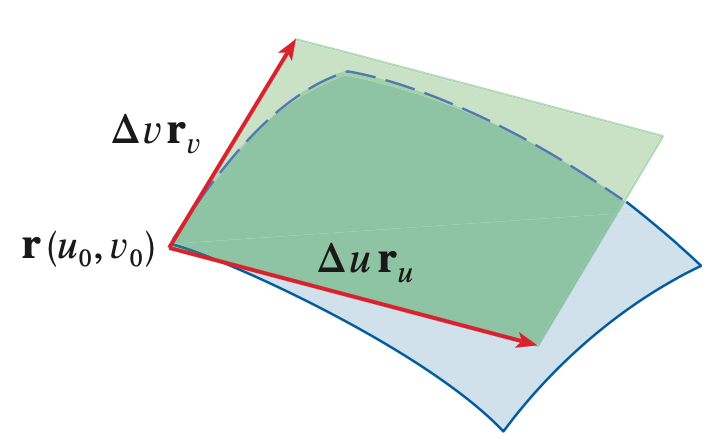
\includegraphics[scale=0.3]{appendices/figures/fig011.png}
    \caption{A change of variables affects a double integral}
\end{figure}

Therefore we can approximate the area of $R$ by the area of this parallelogram, which is

\begin{equation}
    |(\Delta u r_u) \times (\Delta v r_v)| = |r_u \times r_v| \Delta u \Delta v
\end{equation}

Computing the cross product, we obtain

\begin{align*}
    \vec{r_u} \times \vec{r_v} = 
    \begin{vmatrix}
        \mathbf{i} & \mathbf{j} & \mathbf{k}\\
        \frac{\partial x}{\partial u} & \frac{\partial y}{\partial u} & 0\\
        \frac{\partial x}{\partial v} & \frac{\partial y}{\partial v} & 0
    \end{vmatrix}
     = 
     \begin{vmatrix}
        \frac{\partial x}{\partial u} & \frac{\partial y}{\partial u}\\
        \frac{\partial x}{\partial v} & \frac{\partial y}{\partial v}
    \end{vmatrix}
    \mathbf{k} =
     \begin{vmatrix}
        \frac{\partial x}{\partial u} & \frac{\partial x}{\partial v}\\
        \frac{\partial y}{\partial u} & \frac{\partial y}{\partial v}
    \end{vmatrix}
    \mathbf{k}
\end{align*}

The determinant that arises in this calculation is called the \textbf{Jacobian}

\begin{definition}
    The Jacobian of transformation T given by $x=g(u, v)$ and $y=h(u, v)$ is
    
    \begin{align*}
    \frac{\partial(x, y)}{\partial (u, v)} = 
     \begin{vmatrix}
        \frac{\partial x}{\partial u} & \frac{\partial x}{\partial v}\\
        \frac{\partial y}{\partial u} & \frac{\partial y}{\partial v}
    \end{vmatrix}
    =
    \frac{\partial x}{\partial u} \frac{\partial y}{\partial v} - \frac{\partial x}{\partial v}\frac{\partial y}{\partial u}
    \end{align*}
\end{definition}

\begin{definition}
    Suppose that $T$ is a $C^1$ transformation whose Jacobian is nonzero and that $T$ maps a region $S$ in the $uv$-plane onto a region R in the $xy$-plane. Suppose that $f$ is continuous on $R$ and that $R$ and $S$ are type I and type II plane regions. Suppose also that $T$ is one-to-one, except perhaps on the boundary of $S$. Then
\end{definition}

\begin{align*}
    \iint_{R} f(x, y)dA = 
    \iint_{S}f(x(u, v), y(u, v))
    \begin{vmatrix}
        \frac{\partial(x, y)}{\partial (u, v)}
    \end{vmatrix}
  dudv
\end{align*}
